\documentclass[twocolumn,11pt]{abst}




% タイトル
\title{位置センサを使用しない位置制御の研究}

\author{高倉啓祐$\cdot$中野晋(指導教員 伊藤恒平)}

%\urlstyle{rm}

\setcounter{page}{9}
\lhead{}
\chead{}
\rhead{{\sf 16・205}\\{\bf 機械工学科}}
\lfoot{}
%\cfoot{{\sf-\ M-\thepage \ -}}
\cfoot{
 \ifnum \value{page} < 10
  {\sf-\ M-0\thepage \ -}
 \else%
  {\sf-\ M-\thepage \ -}
 \fi%
}
\rfoot{}
\renewcommand{\headrulewidth}{3pt}
%\renewcommand{\footrulewidth}{1pt}



\begin{document}
%\layout
\maketitle
\thispagestyle{fancy}
\pagestyle{fancy}

\setlength{\baselineskip}{5.6truemm}
\kanjiskip=.07zw plus 3pt minus 3pt
\xkanjiskip=.07zw plus 3pt minus 3pt


% 本文

\section{はじめに}
\subsection{研究の背景}
当研究室では高専ロボコンに出場するためのロボットを設計・製作を行っており,今年度はプラ段ボールを高く積み上げるための積込ロボットの製作を行った.この積込ロボットに搭載されているリフト(図\ref{fig:lift})を,コストのかかるセンサを使用せずに任意の高さで停止させたいと考えた.

\begin{figure}[htbp]
  \begin{center}
    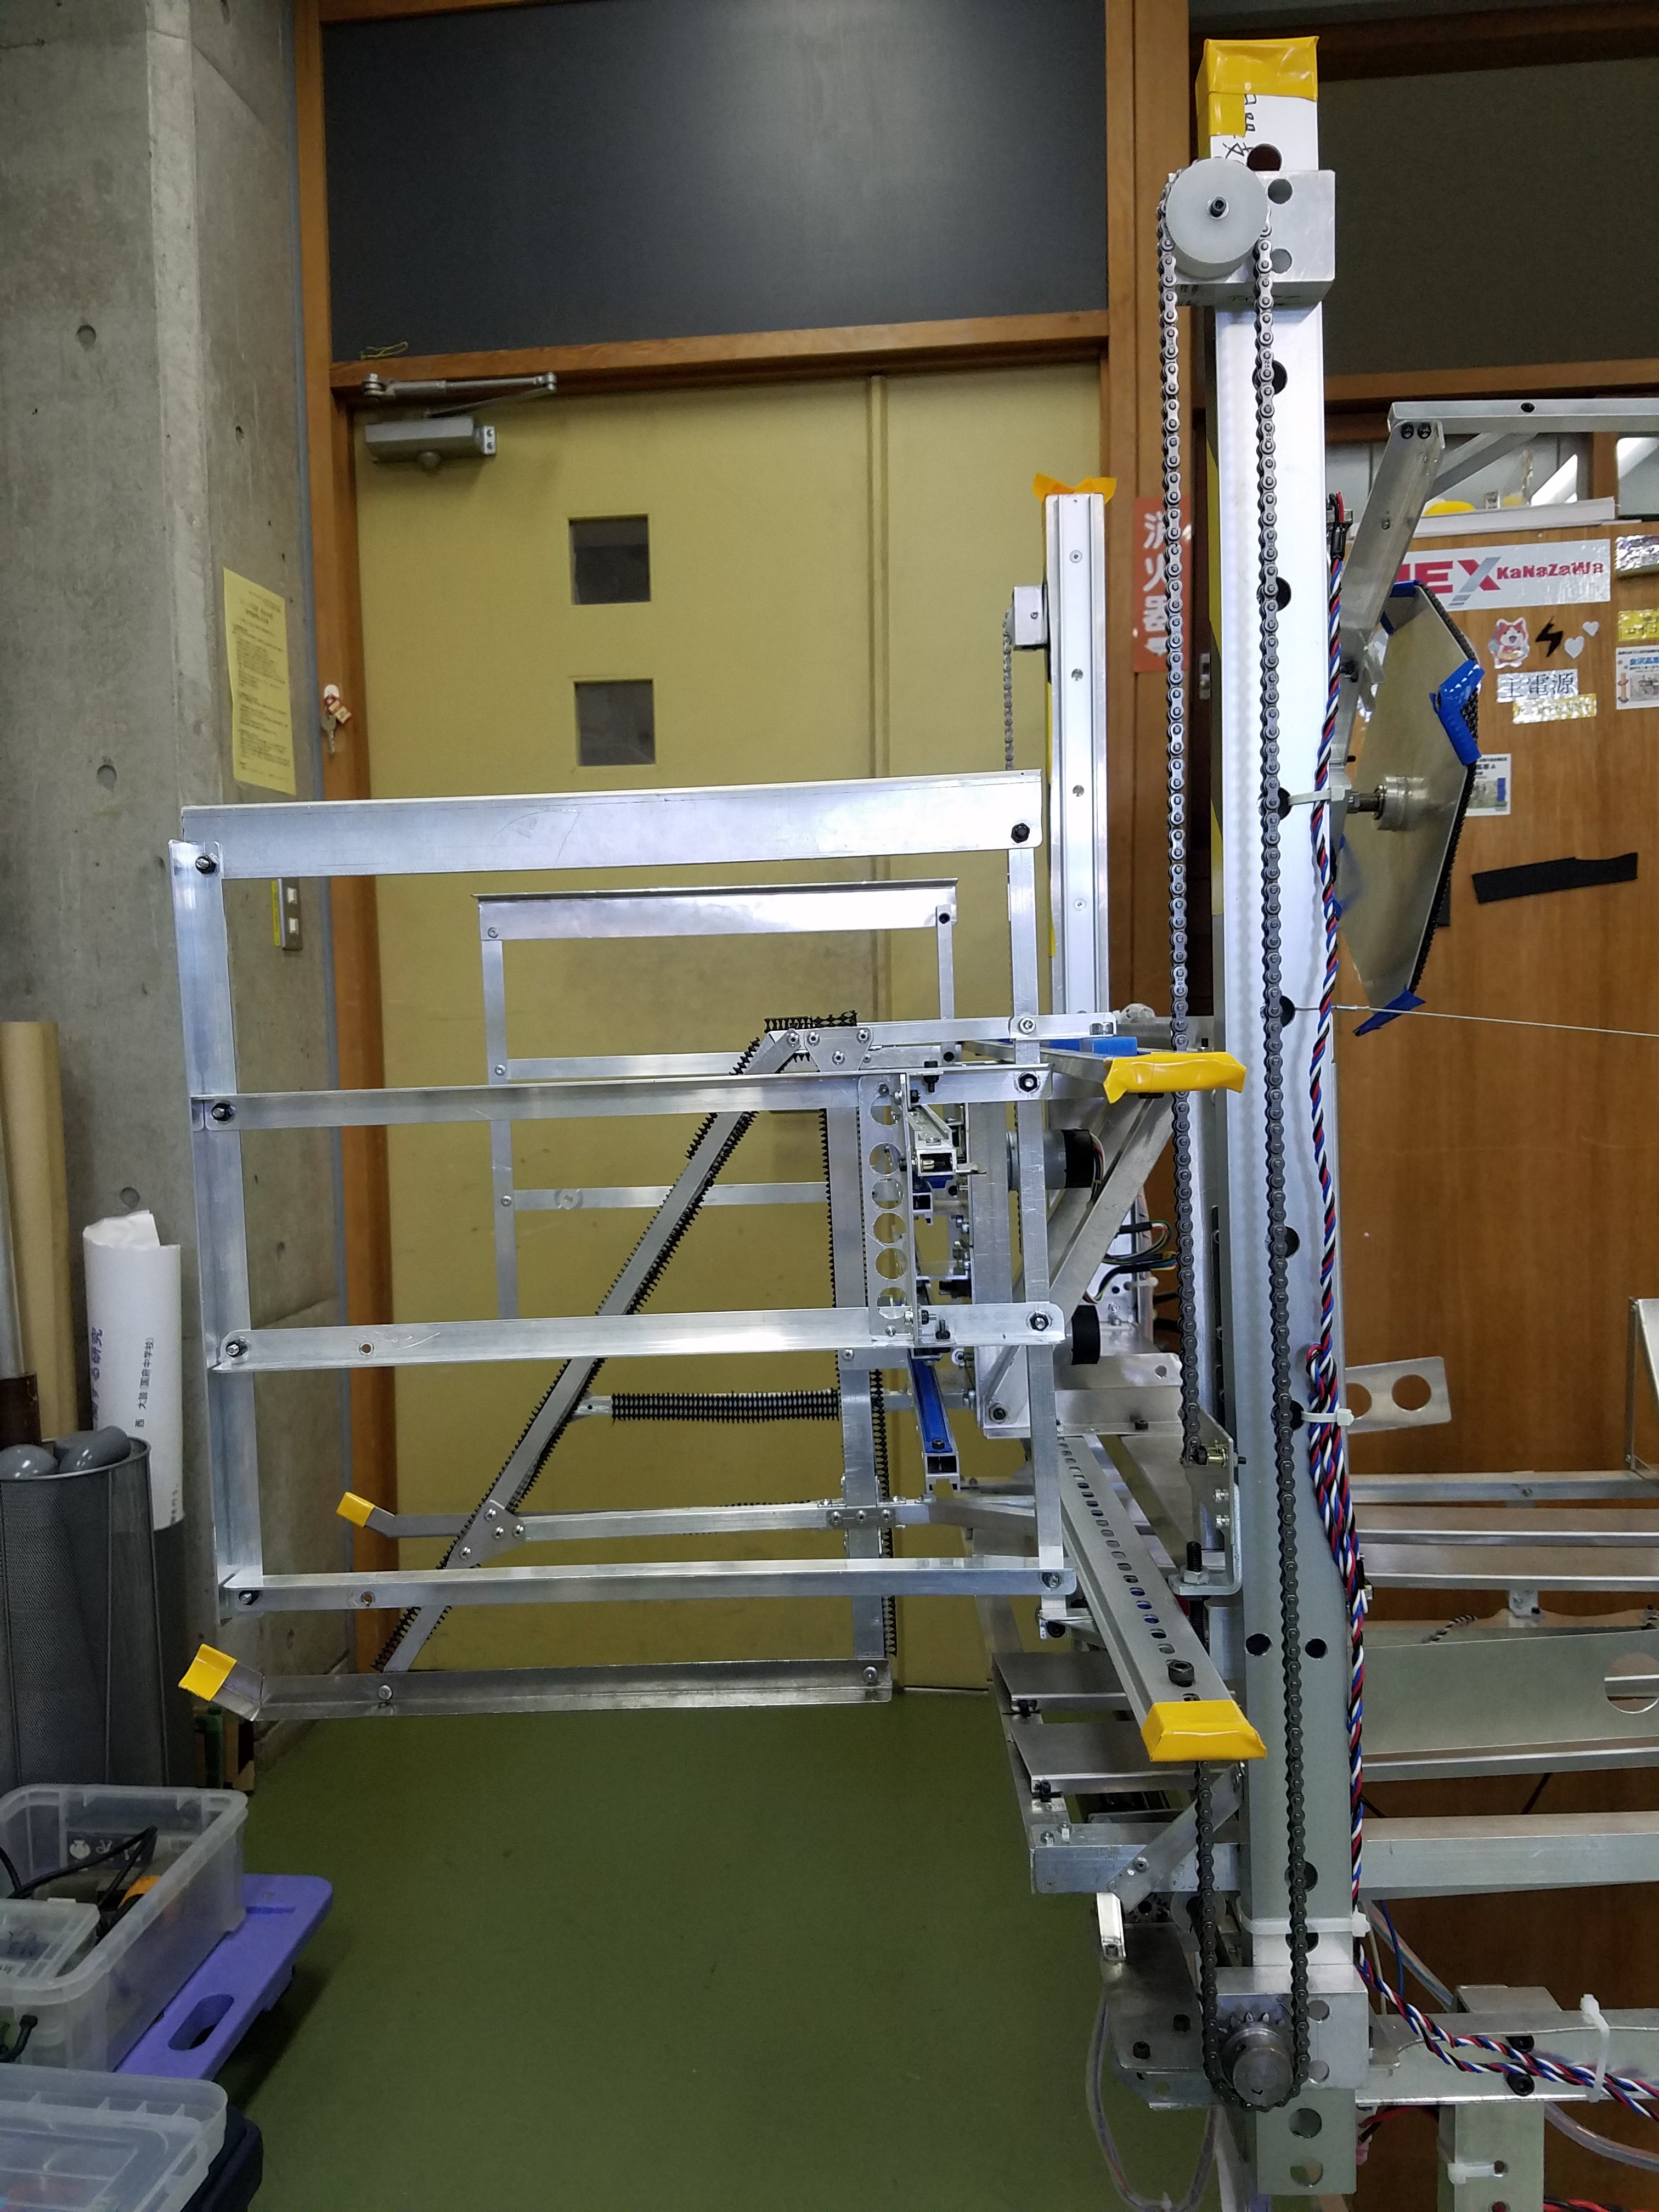
\includegraphics[width=30mm]{img/lift.jpg}
    \end{center}
  \caption{積み込みロボットのリフト}
 \label{fig:lift}
\end{figure}

\subsection{研究の目的}
ロータリーエンコーダといった,直接位置を検出できるセンサを使用せずにリフトを任意の位置に停止させる制御を考案する.

\section{位置制御}
位置制御とは,制御対象の現在位置を何らかのセンサなどで検出し,目標の位置になるように操作する制御である.

\subsection{位置の検出}
モータを動力とする位置制御をする際は,ロータリーエンコーダでモータの回転角度を検出することで制御対象の位置を特定する.このように,位置制御を行う際は位置を直接取得できるセンサを使用して,その値をフィードバックするのが一般的である.

\subsection{制御手法}
\subsubsection{PID制御}
偏差(目標値と現在値の差)に比例して制御量が増える比例制御(P),偏差がある状態が長時間続くにつれ制御量が増えていく積分制御(I),偏差が急激な変化をするほど制御量が増える微分制御(D)を組み合わせた基本的な制御手法である.
\subsubsection{極配置法}
制御対象にはそれぞれ極があり,その値によって応答速度や行き過ぎ量などの特性が変化する.極は状態量を入力にフィードバックすることで変化させることができる.極を望ましい値に設定するフィードバックゲインを探る方法を極配置法という.

\section{センサレス制御}

\subsection{センサレス制御の有効性}
今回のリフトのような位置制御では通常ロータリーエンコーダを使用する.しかし,ロータリーエンコーダを使用するにはそれ専用の取付部を設計するか,既に一体化しているモータを使用する必要があるため,後から取り付ける場合は金銭的,時間的にコストがかかる場合が多い.今回提案する位置制御が実現できればそれらのコストを減らすことができる.

\subsection{制御方法}
モータの電流,電圧,回転速度には関係があり,二つの値が定まるともう一つの値も定まる.電流の値が取得できれば,モータの回転速度を求め,積分して回転角度が求まる.必要なものは電流計測回路のみなので後付けは簡単である.

\subsubsection{制御対象のモデル}
リフトの簡略モデルを図\ref{fig:liftModel}に示す.リフトの運動方程式は式(\ref{eq:lift})のようになる.モータ回路の簡略モデルを図\ref{fig:circuitModel}に示す.モータの運動方程式は式(\ref{eq:motor})のようになる

\begin{eqnarray}
m\dot{v}=\frac{T}{r}-mg
\label{eq:lift}
\end{eqnarray}

\begin{eqnarray}
\begin{array}{l}
RI+K{\omega}=c\\
J\dot{\omega}+\frac{D}{n}{\omega}-\frac{T}{n}=KI
\end{array}
\label{eq:motor}
\end{eqnarray}

\begin{figure}[htbp]
  \begin{center}
    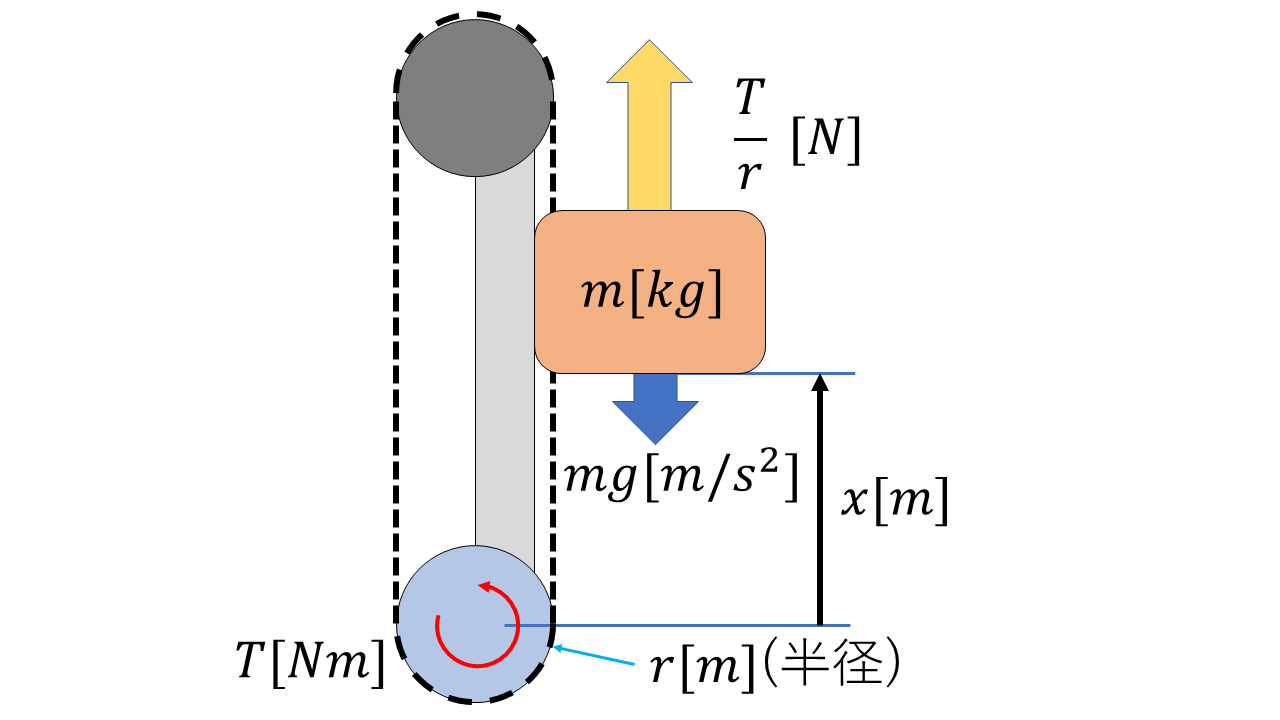
\includegraphics[width=75mm]{img/liftModel.png}
    \end{center}
  \caption{リフトの簡略モデル}
 \label{fig:liftModel}
\end{figure}

\begin{figure}[htbp]
  \begin{center}
    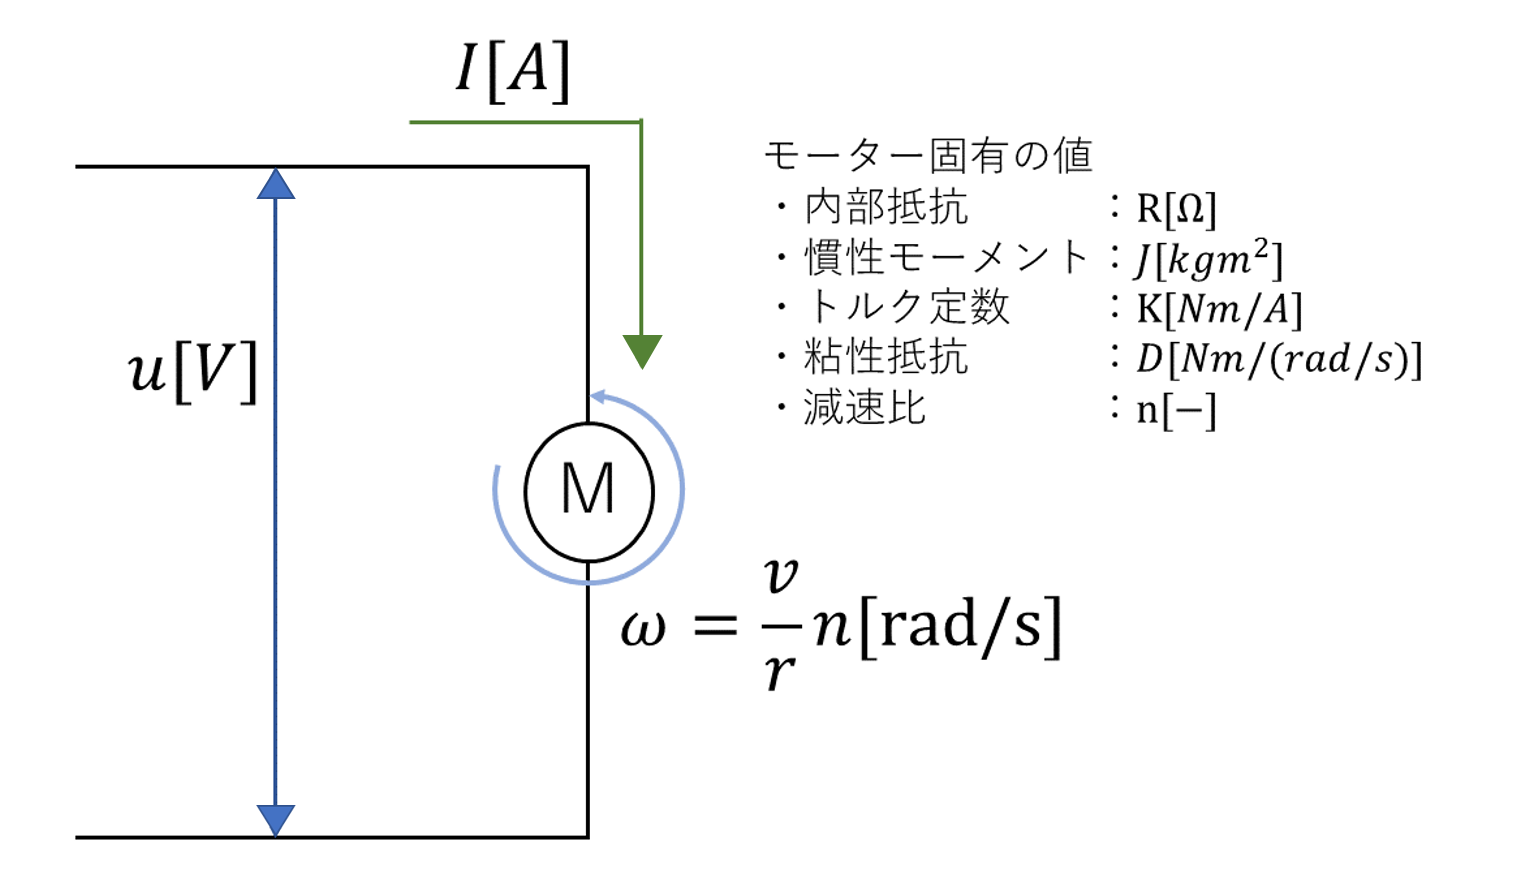
\includegraphics[width=80mm]{img/circuitmodel.png}
    \end{center}
  \caption{モータ回路簡略モデル}
 \label{fig:circuitModel}
\end{figure}

リフトの上昇速度を状態量に,電流値を観測方程式とする状態方程式を立てる.式(\ref{eq:lift}),式(\ref{eq:motor})より,リフトの状態方程式は式(\ref{eq:system})のようになる.

\begin{eqnarray}
\begin{array}{l}
\dot{v}=-\frac{RD+K^2}{RJ+r^{2}m/n^2}v+\frac{KRn}{RJn^{2}+r^{2}m}u-\frac{g}{Jn^{2}/r^{2}m+1}\\
I=-\frac{Kn}{Rr}x+\frac{1}{R}u
\end{array}
\label{eq:system}
\end{eqnarray}

\subsubsection{制御系設計}
ブロック線図を図\ref{fig:blocksenzu}に示す.

\begin{figure}[htbp]
  \begin{center}
    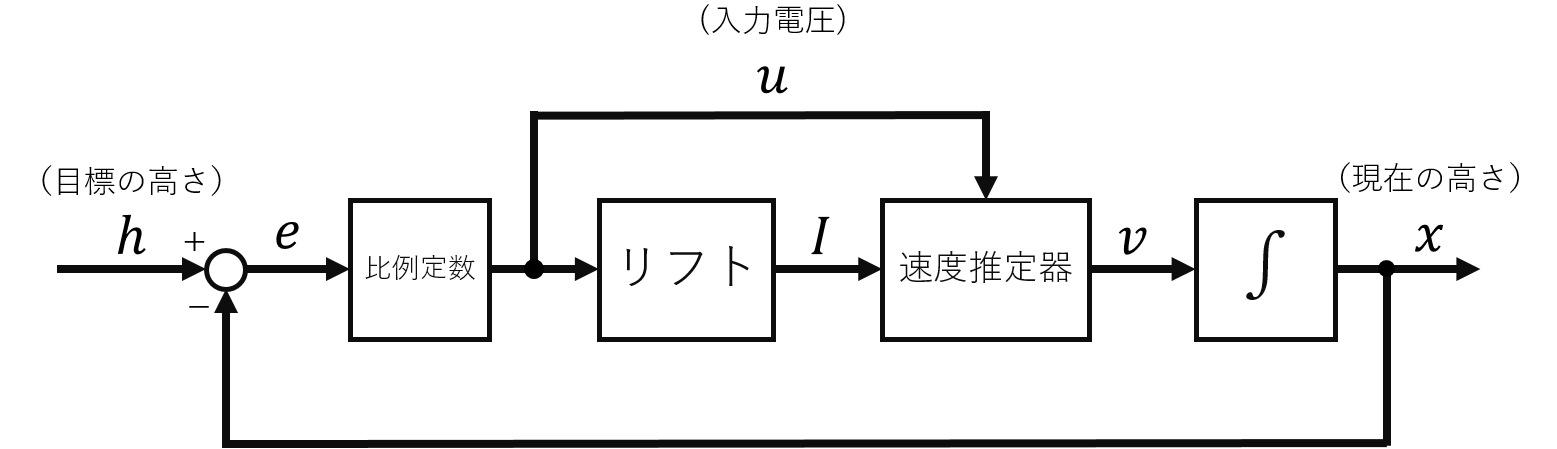
\includegraphics[width=75mm]{img/blocksenzu.png}
    \end{center}
  \caption{ブロック線図}
 \label{fig:blocksenzu}
\end{figure}

リフトの出力する電流と入力の電圧から速度を求め,それを積分して現在値とする.リフトには,目標値と現在値の偏差に比例した値を入力する比例制御を行っている.

\section{シミュレーション}
設計した制御系の性能をシュミレーションで確認する.

\subsubsection{シミュレーションソフト}
シミュレーションには数値計算ソフト「Scilab」に付属しているビジュアルモデリングソフト「Xcos」を使用する.%Xcosで組み立てたブロック線図を図\ref{fig:blockXcos}に示す.

%\begin{figure}[htbp]
%  \begin{center}
%    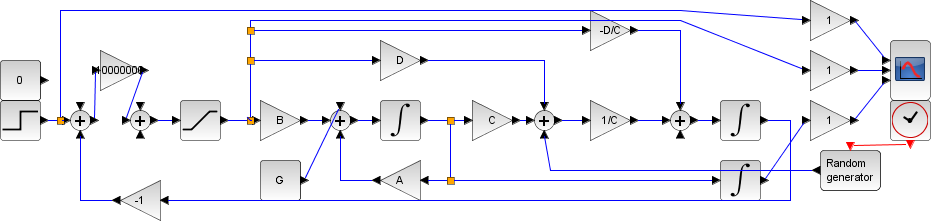
\includegraphics[width=60mm]{img/blockXcos.png}
%    \end{center}
%  \caption{Xcosで組み立てたブロック線図}
% \label{fig:blockXcos}
%\end{figure}

\subsubsection{シミュレーション結果}
シミュレーションの結果を図\ref{fig:sim}に示す.

\begin{figure}[htbp]
 \begin{center}
    \includegraphics[width=80mm]{img/sim.bmp}
    \end{center}
  \caption{入力した目標値による電圧と位置の時間変化}
 \label{fig:sim}
\end{figure}

\section{おわりに}
シミュレーションを使用して,センサレス制御が可能であることを確認することができた.実際のリフトに適用する際には,モータのモデル化誤差と電流検出ノイズによって引き起こされるドリフトを解決する必要があると考えられる.

% 参考文献
\begin{thebibliography}{8}
\bibitem{ob} 熊谷正朗,状態フィードバックとオブザーバ,www.mech.tohoku-gakuin.ac.jp\slash{}rde\slash{}contents\slash{}course\slash{}controlII\slash{}statefeedback.html,2011\slash{}02\slash{}10
\bibitem{sei} 明石 一・今井弘之,制御工学演習,共立出版,2014\slash{}04\slash{}15
\end{thebibliography}


\end{document}